
%%%%%%%%%%%%%%%%%%%%%%%%%%%%%%%%%%%%%%%%%%%%%%%%%%%%%
\section{THz interaction with matter}
%%%%%%%%%%%%%%%%%%%%%%%%%%%%%%%%%%%%%%%%%%%%%%%%%%%%%
This entire work lays its foundations upon Maxwell's macroscopic equations:

\begin{multicols}{2}
\begin{equation}
\nabla \cdot \mathbf{D} = \rho_f,
\label{eq:max1}
\end{equation}
\begin{equation}
\nabla \cdot \mathbf{B}=0,
\label{eq:max2}
\end{equation}
\begin{equation}
\nabla \times \mathbf{E}=-\frac{\partial \mathbf{B}}{\partial t},
\label{eq:max3}
\end{equation}
\begin{equation}
\nabla \times \mathbf{H}=\frac{\partial \mathbf{D}}{\partial t} + \mathbf{J}_f,
\label{eq:max4}
\end{equation}
\end{multicols} \noindent
where $\rho_f$ and $\mathbf{J}_f$ are respectively the free charge and current densities within some space. The macroscopic fields $\mathbf{D}$ and $\mathbf{H}$ are defined as
\begin{multicols}{2}
\begin{equation}
\mathbf{D} \equiv \epsilon_0 \mathbf{E} + \mathbf{P}=\epsilon \mathbf{E},
\label{eq:D definition}
\end{equation}
\begin{equation}
\mathbf{H} \equiv \frac{1}{\mu_0}\mathbf{B} - \mathbf{M}=\frac{1}{\mu}\mathbf{B},
\label{eq:H definition}
\end{equation}
\end{multicols} \noindent
where $\epsilon_0$ and $\mu_0$ are respectively the permittivity and permeability of free space with $\epsilon$ and $\mu$ being the electric permittivity and the magnetic permeability of a material, respectively. The polarization $\mathbf{P}$ and magnetization $\mathbf{M}$ hold the macroscopic information regarding the properties of the medium in mind. 



\subsubsection{Boundary Conditions at a surface discontinuity\label{s2:BCs}}
The above equations are stated for regions of space where there is no discontinuity in the material properties of the medium. However, objects exist causing abrupt changes in the material properties needed to describe the scene in mind. These changes impose boundary conditions to the electric and magnetic fields across the surface of such discontinuities. These boundary conditions are only stated here due to their immense importance in all electro-magnetic phenomena and for the sake of completeness;
\begin{multicols}{2}
\begin{equation}
\mathbf{n}_{12}\cdot (\mathbf{B}^{(2)}-\mathbf{B}^{(1)})=0,
\label{eq2:BC1}
\end{equation}
\begin{equation}
\mathbf{n}_{12}\cdot (\mathbf{D}^{(2)}-\mathbf{D}^{(1)})=\rho_s,
\label{eq2:BC2}
\end{equation}
\begin{equation}
\mathbf{n}_{12}\times (\mathbf{H}^{(2)}-\mathbf{H}^{(1)})=\mathbf{j}_s,
\label{eq2:BC3}
\end{equation}
\begin{equation}
\mathbf{n}_{12}\times (\mathbf{E}^{(2)}-\mathbf{E}^{(1)})=0,
\label{eq2:BC4}
\end{equation}
\end{multicols} 
\noindent where $\rho_s$ and $\mathbf{j}_s$ are respectively the surface charge and current densities across the discontinuity and $\mathbf{n}_{12}$ is the vector normal to the surface. In words, these boundary conditions can be stated as: \textit{The normal component to the magnetic induction and the tangential electric field are both continuous across the discontinuity, and the normal electric displacement and tangential magnetic fields change abruptly with their discontinuities respectively equaling $\rho_s$ and $\mathbf{j}_s \times \mathbf{n}_{12}$.} A full derivation of these boundary conditions can be found in chapter 1.1.3 of ref. \cite{Wolf.Optics}.





%%%%%%%%%%%%%%%%%%%%%%%%%%%%%%%%%%%%%%%%%%%%%%%%%%%%%%%%%
\subsection{Wave equation and Fabry-Perot\label{sec:Wave equation}}
%%%%%%%%%%%%%%%%%%%%%%%%%%%%%%%%%%%%%%%%%%%%%%%%%%%%%%%%%
From Maxwell's equations, we next obtain the wave equation for the electric field. This is accomplished by putting eqs. \eqref{eq:max4}, \eqref{eq:D definition} \& \eqref{eq:H definition} into the curl of eq. \eqref{eq:max3} and simplifying with the vector identity $\nabla \times (\nabla \times \mathbf{A})=\nabla(\nabla \cdot \mathbf{A})-\nabla^2 \mathbf{A}$;
\begin{equation}
\nabla^2 \mathbf{E}-\epsilon \mu \frac{\partial^2 \mathbf{E}}{\partial t^2}=\mu \frac{\partial \mathbf{J}_f}{\partial t}+ \frac{1}{\epsilon}\nabla \rho_f.
\label{eq:pre wave eqn}
\end{equation}
Further simplifications are made with Ohm's law $\mathbf{J}_f=\sigma\mathbf{E} $ and neglecting charge density fluctuations, ie. $\nabla\rho_f=0$, to then obtain
\begin{equation}
\nabla^2 \mathbf{E}-\epsilon \mu \frac{\partial^2 \mathbf{E}}{\partial t^2}=\sigma \mu \frac{\partial \mathbf{E}}{\partial t},
\label{eq:wave eqn}
\end{equation}
where $\sigma$ is the electrical conductivity. An identical wave equation is obtained is for $\mathbf{H}$ in an identical manner. In the case of free space propagation, $\sigma=0, \; \epsilon=\epsilon_0, \; \mu=\mu_0$, one obtains $c=1/\sqrt{\epsilon_0\mu_0}$ as the speed at which an electromagnetic wave moves through a vacuum. In other words $c$ is the speed of light. However, should $\sigma=0$, $\epsilon \neq \epsilon_0$ and $\mu \neq \mu_0$ then the wave propagates with speed $v=c/n$ where $n$ is the refractive index of the material given by $n^2=\frac{\epsilon \mu}{\epsilon_0 \mu_0}$.


Having an equation only sets up the problem and does not yield insight or information regarding the observable world. For this reason, we look for solutions to the wave equation that are expressed as linearly polarized, monochromatic, plane waves traveling in the z-direction with wave-vector $\mathbf{k}=k_z \mathbf{\hat{z}}$, ie:
\begin{equation}
\mathbf{E}(\mathbf{r},t)=\mathbf{E}_0 e^{i(k_z z- \omega t)}.
\label{eq:E plane wave}
\end{equation}
Putting this equation into eq. \eqref{eq:wave eqn} yields the following dispersion relation
\begin{equation}
k^2_z=\omega \mu(\epsilon \omega + i \sigma).
\label{eq:gen. dispersion}
\end{equation}
This relationship determines how a wave propagates in a medium with specific electromagnetic properties $\epsilon, \mu, \sigma$. In the case of a dielectric or an insulator $\sigma \simeq 0$ hence $k_z$ is purely real. Then the wave propagates as
\begin{equation}
\mathbf{E}(\mathbf{r},t)=\mathbf{E}_0 e^{i(\omega \sqrt{\mu \epsilon} z- \omega t)}
\label{eq:real propagation}
\end{equation}
and experiences no decay provided $\mu$ and $\epsilon$ are both positive and real. In a conductor, however, the conductivity is very large such that $\sigma \gg \epsilon \omega$ thus $k^2 \approx i \omega \mu \sigma$. Evidently
\begin{equation}
k=k_r+i k_i \approx \sqrt{\frac{\omega \mu \sigma}{2}}(1+i),
\label{eq:k conductor}
\end{equation}
where $k_r$ and $k_i$ are the real and imaginary parts of the $k$ vector. In this case the EM wave propagates as
\begin{equation}
\mathbf{E}(\mathbf{r},t)=\mathbf{E}_0 e^{i(\omega \mu \sigma z/2- \omega t)}e^{-z/d},
\label{eq:real propagation}
\end{equation}
where $d=\sqrt{\frac{2}{\omega \mu \sigma}}$ is known as the attenuation length or skin depth. This value indicates how far the wave will penetrate before being attenuated.



\subsubsection{Reflections at Boundaries}\label{sec:fresnel}
We now have a plane wave as a simple solution to our wave equation. If we input this into $\nabla \cdot \mathbf{E}=0$ and $\nabla \cdot \mathbf{H} =0$ we observe the following relation
\begin{equation}
\mathbf{k} \cdot \mathbf{E}=\mathbf{k} \cdot \mathbf{H}=0.
\label{eq:k transverse}
\end{equation}
This relationship implies that $\mathbf{E}$ and $\mathbf{H}$ are both perpendicular to the direction of travel, hence EM waves are transverse. A consequence of this is that if one considers transmission through an interface between two media of different refractive indices, then the wave can be polarized perpendicular or parallel in regards to the plane incidence (Figure \ref{fig:Fresnel}). This consequence combined with the continuity boundary conditions at the surface, in \S \ref{s2:BCs}, implies that you get different reflection and transmission coefficients depending on how your incident light is polarized.
\begin{figure}[h]\centering
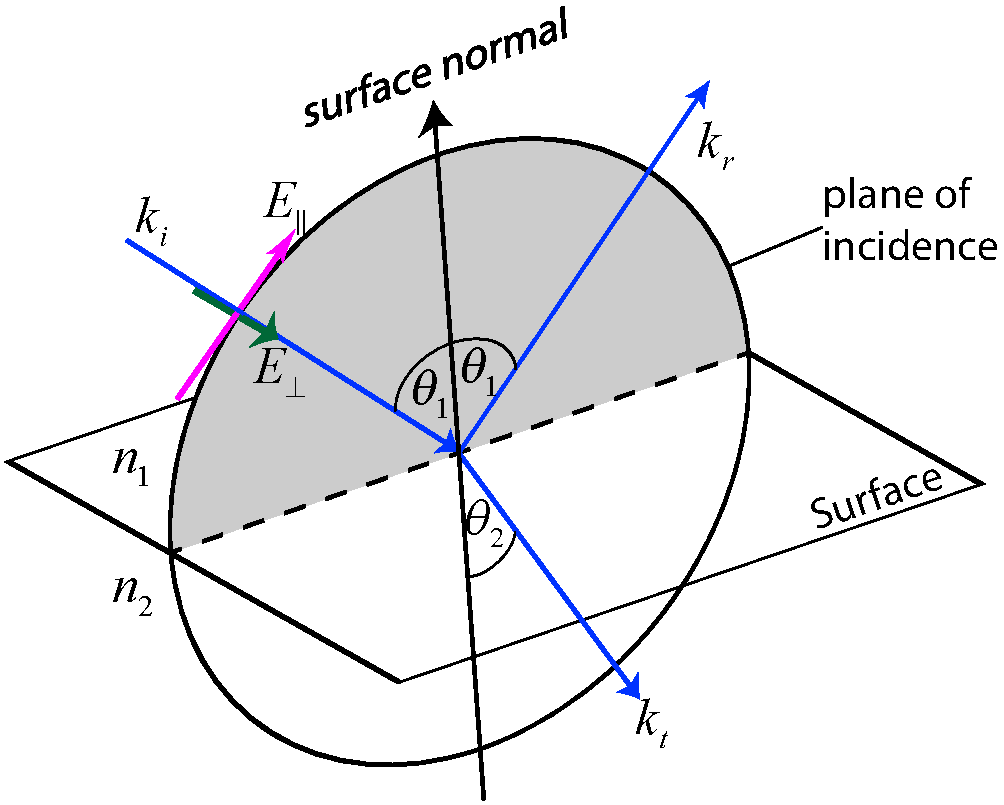
\includegraphics[width=75mm]{Chapters/Theory/Fresnel.pdf}
\caption{Reflection and transmission of a plane wave at a surface between two mediums with different refractive indices. Shown are the incident, reflected and transmitted $k$ vectors in blue, and shown with the pink and green arrows is wave polarization parallel and perpendicular to the plane of incidence respectively.}
\label{fig:Fresnel}
\end{figure}
This fact when combined with Snell's law of refraction
\begin{equation}
n_1 \sin \theta_1=n_2 \sin \theta_2,
\label{eq:Snell's law}
\end{equation}
where $n_{1,2}$ are the refractive indices of the two mediums and $\theta_{1,2}$ are the angles of incidence and refraction, yields the famous Fresnel amplitude reflection and transmission coefficients:
\begin{multicols}{2}
\noindent    %<---- Need this thing!
\begin{equation}
r_{\parallel}=\frac{n_2 \cos \theta_1 - n_1 \cos \theta_2}{n_1 \cos \theta_1 + n_2 \cos \theta_2},  \end{equation}
\begin{equation}
t_{\parallel}=\frac{2n_1 \cos \theta_1}{n_1 \cos \theta_1 + n_2 \cos \theta_2},
\label{eq:Fresnel para}
\end{equation}
\begin{equation}\break
r_{\perp}=\frac{n_1 \cos \theta_1 - n_2 \cos \theta_2}{n_1 \cos \theta_1 + n_2 \cos \theta_2},
\end{equation}
\begin{equation}
t_{\perp}=\frac{2n_1 \cos \theta_1}{n_1 \cos \theta_1 + n_2 \cos \theta_2}.
\label{eq:Fresnel perp}
\end{equation}
\end{multicols} \noindent 
Furthermore one defines the Reflectivity and Transmissivity as $R=|r|^{2}$ and $T=n_2 |t|^2/n_1$.


%%%%%%%%%%%%%%%%%%%%%%%%%%%%%%%%%%%%%%%%%%%%%%%%%%%%%%%%
\subsubsection{Fabry-Perot Interference}\label{sec:Fabry_Perot}
The above consideration would hold absolutely true if our world was made from solely two materials. Obviously untrue, hence the next step of extending our mathematical model of the world is to consider the scenario when the second material is of a finite thickness $L$. When a plane arrives at the incident interface it will split into a reflected and a transmitted component. Then, the transmitted part will come up against the second exit interface and split again. The consequential reflected component will split again at the other interface. This process will carry on going indefinitely. Further, every time the wave travels through the dielectric it will pick up a phase shift, between each preceding member of the set of reflected or transmitted waves, of
\begin{equation}
\phi=\frac{2 \pi f}{c}L n_{2}\cos \theta_2,
\label{eq:phase}
\end{equation}
where $f$ is the frequency of the wave. 
\begin{figure}[h]\centering
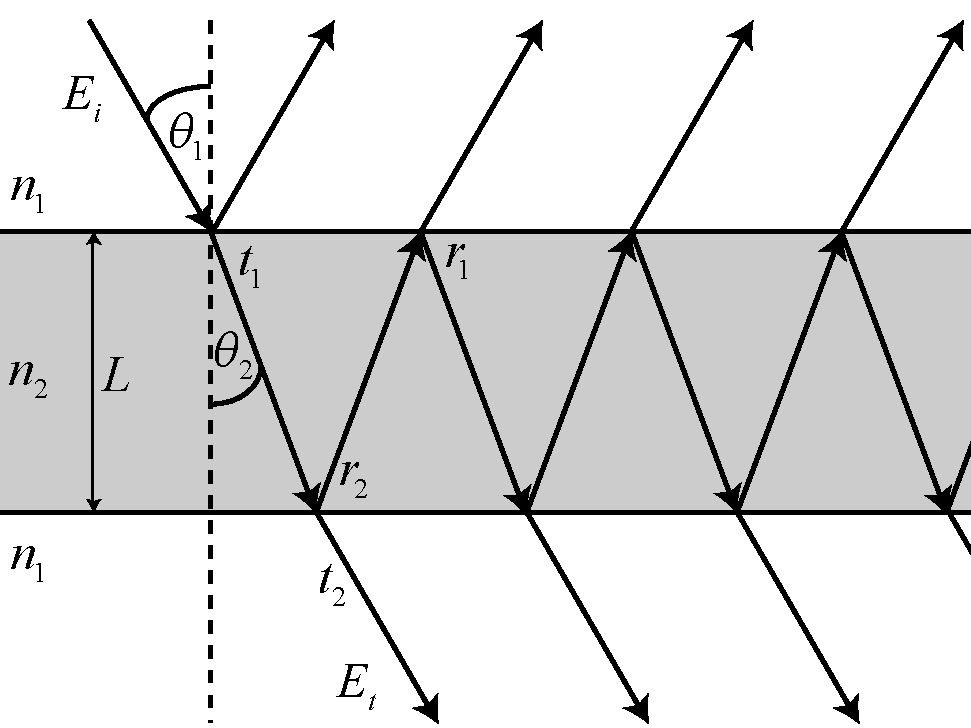
\includegraphics[width=75mm]{Chapters/Theory/Fabry-perot.pdf}
\caption{Reflection and transmission of a plane wave undergoing multiple reflections within a dialectic.}
\label{fig:Fabry-perot}
\end{figure}
A \textit{Fabry-Perot resonance} is defined as when all the components resulting from each individual splitting of the wave interfere constructively. Now, if one considers the superposition of all these waves then the total transmitted field $E_t$ is given by
\begin{equation}
\begin{split}
\begin{split}
E_t&=E_i t_1 t_2e^{i\phi}(1+r_1 r_2 e^{2i\phi}+ r_1^2 r_2^2 e^{4i\phi}+...
\\ &=E_i t_1 t_2 e^{i\phi}\sum_{n=0}^{\infty}(r_1 r_2 e^{2i\phi})^{n}
\\ &=E_i \frac{ t_1 t_2e^{i\phi}}{1 - r_1 r_2 e^{2i\phi}},
\label{eq:Fabry-Perot T}
\end{split}
\end{split}
\end{equation}
where $t_1,\; t_2,\; r_1,\; r_2$ are the relevant Fresnel coefficients in fig. \ref{fig:Fabry-perot}. A more detailed derivation is given in ch. 7.6.1 of ref. \cite{Wolf.Optics} along with the equation for reflection;
\begin{equation}
E_r=-\frac{r_2(1-(r_2^2+t_1 t_2)e^{2i\phi}}{1-r_2^2 e^{2i\phi}}E_i.
\label{eq:Fabry-Perot R}
\end{equation}
These two equations \eqref{eq:Fabry-Perot T} \& \eqref{eq:Fabry-Perot R} do need to be considered if one wishes to do a reflection or transmission experiment through any material. In THz measurements they are also used to extract permittivity of an unknown material, as outlined in \S\ref{sec:multi-layers}.






%%%%%%%%%%%%%%%%%%%%%%%%%%%%%%%%%%%%%%%%%%%%%%%%%%%%%%%%%
\subsection{Fundamental models of matter}
%%%%%%%%%%%%%%%%%%%%%%%%%%%%%%%%%%%%%%%%%%%%%%%%%%%%%%%%%
So far, the previous sub-sections have assumed that the materials properties, $\epsilon, \mu$ and $\sigma$, do not change with the frequency of the EM wave. This is false for all materials in an absolute sense, however for certain frequency ranges this can be approximately true and such materials are called dispersion-less. However, most materials do change with frequency since everything contains atoms and electrons which interact with an incident EM wave. 

%%%%%%%%%%%%%%%%%%%%%%%%%%%%%%%%%%%%%%%%%%%%%%%%%%%%%%%%%%%%%%%
\subsubsection{Classical Lorentzian}
\label{sec2:Classical Lorentzian}
For an improved mathematical description of the world the classical Lorentzian model was developed. It accounts for the response of charged and bound particles to an incident EM wave. Here, one assumes that a bound charge oscillates about its equilibrium position and thus has a potential energy given by a simple harmonic oscillator of frequency $\omega_0$ and mass $m$:
\begin{equation}
U(x)=\frac{1}{2}m \omega_0^2 x^2.
\label{eq:harmonic potential}
\end{equation}
Then the charged particle will experience a restoring force $F_r$ from $\mathbf{F}=-\nabla U$. Further more, there will be a damping term $F_d$ and a force from the incident electric field $F_E$. Combining these forces into Newton's second law gives;
\begin{equation}
\begin{split}
m\frac{d^2 x}{dt^2}&=F_r+F_d+F_E
\\ &=-m\omega_0^2x-m\gamma\frac{dx}{dt}+qE,
\label{eq:Newton 2nd law}
\end{split}
\end{equation}
where $\gamma$ is the phenomelogical damping rate and $q$ is the charge of the charged particle. If we say that we have a scalar monochromatic linearly polarized EM wave, ie. it is of the form of eq. \eqref{eq:E plane wave}, then the solution to eq. \eqref{eq:Newton 2nd law} is given by
\begin{equation}
x(t)=\frac{q E_0 e^{-i\omega t}}{m(\omega_0^2-\omega^2-i\gamma\omega)}.
\label{eq:linear harmonic oscillation}
\end{equation}
Now one knows the electric dipole moment per charged harmonic oscillator $p(t)=qx(t)$. Hence, for a medium with $N$ oscillators per unit volume we have an electric polarization of
\begin{equation}
P(t)=Nqx(t)=\frac{Nq^2 E_0 e^{-i\omega t}}{m(\omega_0^2-\omega^2-i\gamma\omega)}\equiv \epsilon_0 \chi(\omega)E_0 e^{-i\omega t},
\label{eq:Lorentz oscillator}
\end{equation}
where $\chi(\omega)$ is the linear susceptibility of the medium. Now if we consider eqs. \eqref{eq:D definition} and \eqref{eq:Lorentz oscillator} we can define the relative permittivity of our medium
\begin{equation}
\epsilon_r (\omega) \equiv \frac{\epsilon(\omega)}{\epsilon_0} =1 + \chi(\omega)=1 + \frac{Nq^2 }{m\epsilon_0(\omega_0^2-\omega^2-i\gamma\omega)}
\label{eq:relative permittivity}
\end{equation}
with real and imaginary parts $\epsilon_r=\epsilon_r'+i\epsilon_r''$, given by
\begin{equation}
\epsilon_r'=\frac{Nq^2(\omega_0^2-\omega^2)}{m\epsilon_0((\omega_0^2-\omega^2)+\omega^2\gamma^2)}
\label{eq:epsilon real}
\end{equation}
\begin{equation}
\epsilon_r''=\frac{Nq^2\omega\gamma}{m\epsilon_0((\omega_0^2-\omega^2)+\omega^2\gamma^2)}
\label{eq:epsilon imaginary}
\end{equation}
In terahertz this model is most often used to account for the absorption caused by crystal lattice vibrations.


%%%%%%%%%%%%%%%%%%%%%%%%%%%%%%%%%%%%%%%%%%%%%%%%%%%%%
\subsubsection{Drude model}
\label{sec:Drude Model}
In the section above the charged particle is bound in space, however the scenario of it being free to move about in space is also possible. To account for such a response the Drude model was developed. Its assumptions are that we have a sea of mobile electrons and a set of stationary positively charged ions constituting our medium. The mobile electrons freely move in only straight lines unaffected by any other forces except those in the instantaneous (assumed to be so) collisions with the impenetrable ion cores (electron-electron collisions conserve momentum hence no change to the current). The electrons collide with the ion cores on average after time $\tau$. This is the only mechanism by which they reach thermal equilibrium, hence we assume that each collision randomizes the velocity with a speed appropriate to the local thermal conditions.


With the above assumptions we can find the DC electrical conductivity of a material. This is done by considering the current density created from $N$ electrons per unit volume moving through a surface area perpendicular to velocity of the electrons $\mathbf{v}$. The charge carried by each electrons is $-e$, hence the current density is simply 
\begin{equation}
\mathbf{J}=-Ne\mathbf{v}.
\label{eq:Drude current}
\end{equation}
Now, if we apply an electric field $\mathbf{E}$ then after time $t$ an electron's velocity will be $\mathbf{v}=\mathbf{v}_0-e\mathbf{E}t/m$, where $\mathbf{v}_0$ is the electron's velocity after its previous collision. Due to the velocity randomization through each collision $\mathbf{v}_0$ averages out to zero. Since each collision occurs on average after time $\tau$, we have
\begin{equation}
\mathbf{v}_{avg}=-\frac{e\mathbf{E}\tau}{m}; \;\;\;\;\;\; \mathbf{J}=\frac{Ne^2\tau}{m}\mathbf{E},
\label{eq:Drude average}
\end{equation} 
where $\mathbf{v}_{avg}$ is known as the electron drift velocity. From Ohm's law we can see that the DC conducivity, $\sigma_0$, of a metal is
\begin{equation}
 \mathbf{J}=\sigma_0 \mathbf{E}; \;\;\;\;\;\; \sigma_0=\frac{Ne^2\tau}{m}.
\label{eq:Drude conductivity}
\end{equation}
In practice we don't know $\tau$ but by measuring the conductivity we can estimate values for it.


With the above assumptions, the Drude response of a medium to a monochromatic wave can be characterized by that of a Classical Lorentzian oscillator centered at zero frequency and a damping rate equal to the probability of collision per unit time, ie. $\omega_0=0$ and $\gamma=1/\tau$ in eq. \eqref{eq:linear harmonic oscillation}. However, we are interested in the velocity not position so we can use eq. \eqref{eq:Drude current} to obtain
\begin{equation}
\sigma(\omega)=\frac{Ne^2\tau}{m(1-i\omega\tau)}=\frac{\sigma_0}{1-i\omega\tau}
\label{eq:Drude AC conductivity}
\end{equation}
as the AC conductivity of our material. Now, if we turn our attention to the wave equation \eqref{eq:wave eqn} describing our EM wave and say $\mu=\mu_0$, we can see that it can written in the form 
\begin{equation}
\nabla^2 \mathbf{E}=-\omega^2 \mu_0\left(\epsilon+ \frac{i \sigma_0}{\omega(1-i\omega \tau)}\right)\mathbf{E}.
\label{eq:drude wave equation}
\end{equation}
This yields the following dispersion relation for our monochromatic wave; 
\begin{equation}
k_z^2=\omega^2\mu_0 \epsilon_0\epsilon(\omega); \;\;\;\;\; \epsilon(\omega)=\epsilon_{\infty}+\frac{i \sigma_0}{\epsilon_0\omega(1-i\omega \tau)},
\label{eq:drude dispersion}
\end{equation}
where $\epsilon_{\infty}$ is the frequency independent dielectric permittivity due to the contribution of bound charges and $\epsilon(\omega)$ is known as the Drude permittivity.

If we now consider the case of $\omega\tau>>1$ we can see that our Drude permittivity approximates to
\begin{equation}
\epsilon(\omega)=\epsilon_{\infty}-\frac{Ne^2}{m\epsilon_0\omega^2}=\epsilon_{\infty}-\frac{\omega_p^2}{\omega^2},
\label{eq:plasma frequency}
\end{equation}
where $\omega_p=\sqrt{Ne^2/m\epsilon_0}$ is known as the plasma frequency of the material. Since $k_z \propto \sqrt{\epsilon(\omega)}$ then when $\omega^2 \epsilon_\infty>\omega_p^2$ we have a purely real dispersion relation thus the wave propagates inside the material. For $\omega^2 \epsilon_\infty<\omega_p^2$ we have a purely imaginary $k_z$ signifying  that the waves decay inside the material at the rate given by $k_i(\omega)=\frac{1}{c}\sqrt{\omega_p^2-\epsilon_\infty\omega^2}$.


%%%%%%%%%%%%%%%%%%%%%%%%%%%%%%%%%%%%%%%%%%%%%%%%%%%%%
\subsubsection{Quantum Models of Charge carriers}
The Free-Electron model was developed to better understand solids and the conduction of electrons through metals. It considers the valence electrons of a material and makes similar assumptions to the Drude model along with taking into account Quantum theory and Pauli's exclusion principle. This model gives insight into the thermal and electrical conductivity, heat capacity and electrodynamics of metals. However, it fails to point out the distinction between metals, semiconductors and insulators. To understand this distinction the Nearly Free-Electron model was developed.

The Nearly Free-Electron model makes a step further by taking into account how the conducting electrons experience a potential energy variation due to the lattice arrangement of the positive ion cores within a crystal. This model gives intuitive insight into the observed band structure of solid matter, in other words why there exist electrons with momentum values which do not propagate through the crystal. This is done by considering the Bragg reflection condition within the first Brillouin zone of the crystal lattice in mind; one sees that two different standing waves can be set up from the periodicity of the lattice. One piles up electrons on top of the positive ions and the other in between the ion cores. Due to the attractive forces between the negative electrons and positive cores, the first wave has a lower total energy. The difference in two energies is known as the energy gap, $E_g$.

The size of the energy gap between the conduction and valance electron bands determines whether a material is a metal, a semiconductor or an insulator as follows; metals have no energy gap hence there is always filled states in the conduction band, semiconductors have a small gap thus it is easy to excite electrons into a conducting state and insulators have a large energy gap hence a lot of energy is required to force electrons to become conducting (shown in Fig. \ref{fig:Band}).
\begin{figure}[h]\centering
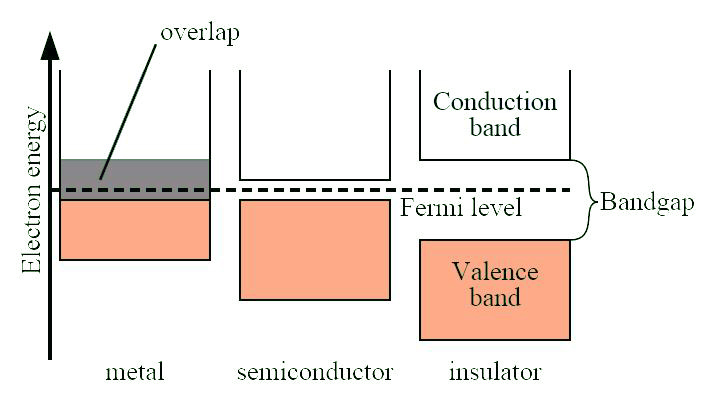
\includegraphics[width=75mm]{Chapters/Theory/band.jpg}
\caption{Band structures of metals, semiconductors and insulators. The Fermi level shows where the electron states are filled up to. Taken from \href{http://cnx.org/content/m43554/latest/graphics2.jpg}{hyperphysics}}
\label{fig:Band}
\end{figure}
Another important feature to consider here is when an electron is excited into the conduction band a vacant orbital is left in the valance band, which is referred to a hole. Holes act though as they are an electron with positive $+e$ charge and mass $m_h=-m_e$ in applied electric and magnetic fields. In other words, they contribute to the overall current within our material. Thus, they are considered as charge carriers along with the electrons. Both these charge carriers do not behave like their counterparts in free-space. To account for this a theoretical simplification is made by saying electrons and holes behave like free-space particles with an effective mass $m^*$.

Next, we define the charge carrier mobility as the magnitude of its drift velocity per unit electric field, ie $\mu=|\mathbf{v}_{avg}|/E$ or $\mu=q\tau/m^*$  from consideration of eq. \eqref{eq:Drude average} \cite{intro_solids}. Then the electrical conductivity of our medium is
\begin{equation}
\sigma=N_e e \mu_e + N_h e \mu_h,
\label{eq:carrier conduction}
\end{equation}
where $\mu_e$ \& $\mu_h$ are the electron and hole mobilities respectively. Further, the conduction electrons and holes will diffuse according to the 3D diffusion equation. Hence, their mean square displacement is
\begin{equation}
<x^2>=6Dt,
\label{eq:diffusion}
\end{equation}
where $D$ is the diffusion coefficient given by the Einstein-Smoluchowski relation, $D=\mu_q k_B T / q$ where $\mu_q$ is the mobility of the charge carrier given earlier in this paragraph. 

%%%%%%%%%%%%%%%%%%%%%%%%%%%%%%%%%%%%%%%%%%%%%%%%%%%%%%%%%
\subsection{Material properties at THz}
%%%%%%%%%%%%%%%%%%%%%%%%%%%%%%%%%%%%%%%%%%%%%%%%%%%%%%%%%

%%%%%%%%%%%%%%%%%%%%%%%%%%%%%%%%%%%%%%%%%%%%%%%%%%%%%
\subsubsection{Conductors}
The terahertz response to highly conductive mediums such as metals is well accounted for by the Drude model. The typical relaxation times of metals are on the order of $10^{-14}$s implying that $\omega \tau <<1$. This reduces $\sigma(\omega)$ and $\epsilon(\omega)$ in eqs. \eqref{eq:drude dispersion} and \eqref{eq:Drude AC conductivity} respectively down to $\sigma(\omega)=\sigma_0$ and $\epsilon(\omega) \approx i \sigma_0/( \epsilon_0 \omega)$. This yields a reflectivity of $R(\omega)\approx1-\sqrt{8\epsilon_0\omega/\sigma_0}$. In the end, typical metals with conductivities on the order of $10^{7}$ S.m$^{-1}$ have a penetration depth of 400 nm and a reflectivity of 98-99\%, table \ref{tab:Metal reflectivity} show reflection values of common metals. Metals are used as THz reflectors.
\begin{table}[h!]
\caption{THz reflectivity of metals, uncertainty $\pm0.1\%$. From \cite{MaterialsatTHz}. }
\centering
\begin{tabular} {c c c}
\hline\hline
Metals & R at 0.58THz & R at 2.55THz\\
\hline
Copper & 0.997 & 1\\
Silver & 0.996 & 0.995\\
Gold & 0.994 & 0.994\\
Aluminium & 0.995 & 0.994\\
Nickel & 0.994 & 0.991\\
Chromium & 0.993 & 0.974\\
\hline
\end{tabular}
\label{tab:Metal reflectivity}
\end{table}


In regards to THz applications, transparent conductors such as tin doped indium oxide (ITO) are very interesting. The visible light transmittance of ITO is reported to be around 90\%. Its conductivity is on the order of $10^6$ S.m$^{-1}$ yielding a reflectivity of 98\% at 1 THz. This allows for the creation of a THz reflector that transmits an optical beam.


%%%%%%%%%%%%%%%%%%%%%%%%%%%%%%%%%%%%%%%%%%%%%%%%%%%%%
\subsubsection{Glass and polymers}
Ordinary glasses exhibit high losses due to charged defects at THz and thus are not used as optical elements. Much more transmissive materials include polymers, dielectrics and semiconductors. Polymers give on average an absorption coefficients around 0.4 cm$^{-1}$ at 1 THz \cite{PrinciplesofTHz} and typical refractive indices of around 1.5 \cite{Terahertzpolymers}. Due to their refractive indices polymers can be used as THz lenses, however their absorption coefficients increase with frequency as shown by Fig. \ref{fig:polymer_absorption}.
\begin{figure}[h!]\centering
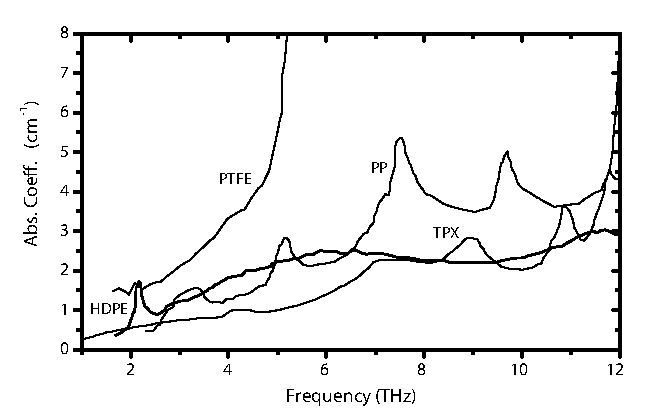
\includegraphics[width=0.70\linewidth]{Chapters/Theory/polymer_absorption.pdf}
\caption{Absorption coefficients of some polymers versus frequency in the range of 2-12 THz. Polymers shown are: High-density polyethylene (HDPE), Teflon (PTFE), Polypropylene (PP) and Polymethylpentene (TPX). Figure from \cite{PrinciplesofTHz}.}
\label{fig:polymer_absorption}
\end{figure}
A mention goes to Tsurupica, a highly transparent polymer for both THz and visible light with a refractive index of 1.52 for both bands.



%%%%%%%%%%%%%%%%%%%%%%%%%%%%%%%%%%%%%%%%%%%%%%%%%%%%%
\subsubsection{Semiconductors}
Silicon is probably going to be one of the most crucial materials for device development at Terahertz frequencies; the reasons are because it's very transmissive, nearly dispersionless and there is an advanced Silicon manufacturing industry which supplies highly quality cheap Silicon quickly, a feature useful for any realistic experimentalist. Further more there is a rich literature regarding its mechanical and electrical properties.

Silicon refractive index was measured to be 3.4175 and to vary by $\pm 0.0001$ over the frequency range of 0.5-4.5 THz. Its absorption coefficient was measured to be 0.04 cm$^{-1}$ at 1 THz \cite{THzsilicon}. Silicon is commonly used in THz lenses. An extra point, the plasma frequency of highly resistive Silicon lies below the terahertz regime. However, by modulation of free charge carrier concentration one can switch the material response from dielectric to conductor (see \S\ref{sec:THz_mod}).

One way of controlling the carrier density is via optical excitation with photons of energy $\hbar \omega$, further discussed in \S \ref{sec:THz_mod}. Reference \cite{Photo.Si} was the first to demonstrate amplitude, phase and frequency modulation of THz via the optical excitation of silicon. More recently, people have built upon these ideas to create an optically modulated wire-grid polarizer \cite{Siopticalpolarizer} and to image objects by creating an imaging mask \cite{Photo.Single} in Silicon. There are other materials which have similar properties such as InSb and GaAs. 





%------------%		IMAGE THEORY		%------------%

\section{Image theory and Fourier Optics}
When light impinges upon an object it is scattered from it in all directions. Then, how this scattered light reaches our eyes, or an external detector, is the prime concern of imaging theory. Rephrased in modern terms, how is a set of EM-field disturbances at point A related to a set at point B. Below is an overview of the theories used for modeling in this thesis.

\subsection{Scalar diffraction theory}\label{sec:scalar_diffraction}
Although light is a vectorial wave, many initial imaging experiments showed remarkable agreeance with scalar diffraction theories. In other words, the Cartesian components of an EM-field are not coupled together, by Maxwells eqs. (\ref{eq:max1}-\ref{eq:max4}), but the behavior of each individual component is summarized by a single scalar wave equation \cite{F.optics}
\begin{equation}
\nabla^2 U(p,t) - \frac{n^2}{c^2}\frac{\partial^2 U(p,t)}{\partial t^2}=0,
\label{eq:scalar_wave}
\end{equation}
where $U(p,t)$ represents the scalar field components at position $p$ and time $t$. Now one needs to impose some boundary conditions describing the object in mind. After solving the resulting equation one can calculate how the field distribution at the object will propagate to any point of observation. However, different theories make various assumptions to obtain a solution. 



Next, we follow the work of ref. \cite{scalar_near_fields}. Therein, by assuming a monochromatic wave and that all scatterers, sources and diffracting apertures are located in negative $z$-space Kowarz obtains a solution to eq. \eqref{eq:scalar_wave} for positive $z$-space. His expression for the electric field $U(x,z)$ is the sum of two parts, a homogeneous propagating field $U_h(x,z)$ and an evanescent field $U_i(x,z)$:
\begin{equation}
U_h(x,z) = \int_{|u_x| \leq 1 }A(u_x) e^{i k u_x x} e^{ikz\sqrt{1-u_x^2}}\text{d}u_x,
\label{eq:U_h}
\end{equation}

\begin{equation}
U_i(x,z) = \int_{|u_x| \geq 1 }A(u_x) e^{i k u_x x} e^{-kz\sqrt{u_x^2-1}}\text{d}u_x,
\label{eq:U_i}
\end{equation}
where $u_x$ is the directional wavevector, $k$ is the free space wavenumber in $x$ and $A(u_x)$ is a spectral amplitude function that is the Fourier transform of the scatterer's field distribution in the plane $z=0$, ie.
\begin{equation}
A(u_x) = \frac{k}{2\pi}\int_{-\infty}^{\infty} U(x,0) e^{-i k u_x x} \text{d}x.
\label{eq:A(u_x)}
\end{equation}
From the above three equations one can calculate the diffraction of a field distribution $U(x,0)$ at any plane in positive $z$ space. Note, the intensity is defined as $I(x,z)  \equiv |U(x,z)|^2 = |U_h(x,z) + U_i(x,z)|^2$. 

A technical note, in our experiments we have multiple frequencies. To account for this, we sum the diffracted fields for all our frequencies, where each frequency component has an input amplitude given by our pulse spectrum (fig. \ref{fig:THz_TDS}\textbf{B}) and a silicon equivalent wavelength. Finally, for ch. \ref{c:mod_thick} we extend this theory to two dimensions by considering the 2D Fourier transform of eq. \ref{eq:A(u_x)} and adding an extra integral over $u_y$\footnote{Note the square root terms become $\sqrt{1 - u_x^2 - u_y^2}$ and there is an extra $e^{iku_y y}$ term.} in eqs. \ref{eq:U_h} \& \ref{eq:U_i}.  



% - - - - - 	MODAL MATCHING		- - - - - %
\subsection{Vectorial modal matching theory}\label{sec:modal_matching}
It is always of preference to use simpler mathematical models to describe the world. However, these usually come with assumptions and restrictions rendering them unusable in certain scenarios. Namely, polarization effects are neglected by the scalar diffraction approximation in the above section. For this reason, next follows an outline of a full wave modal matching solution to Maxwell's equations. Note that this theory was used in Ch. \ref{c:1D_slit} and \ref{c:cartilage}, however the method is outlined using the simpler equations of Ch. \ref{c:cartilage}.  

\begin{figure}[ht]
\centering
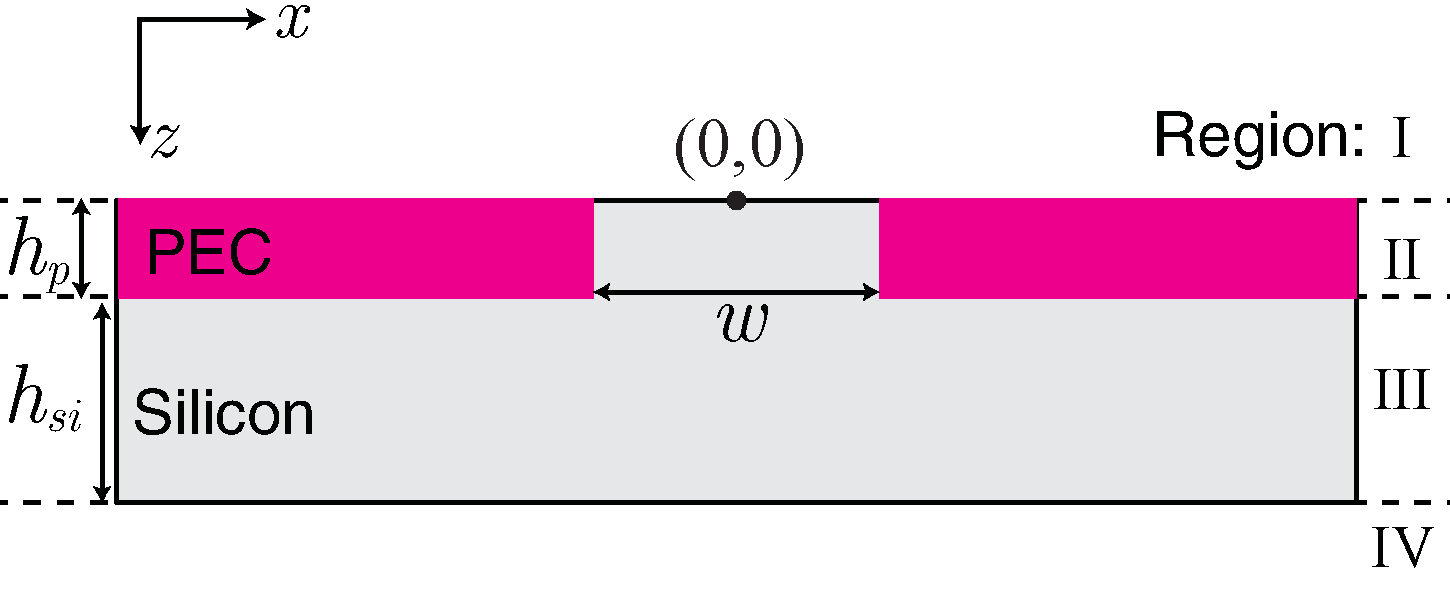
\includegraphics[width=0.65\linewidth]{Chapters/Theory/Modal_sample.pdf}
\caption{Schematic showing the variable definitions used in the modal matching calculations of Sec. \ref{sec:modal_matching}. $h_p=11\mu$m is the penetration depth of  our 800nm pump light \cite{si_depth}, $h_{si}=104\mu$m is the thickness of our silicon wafer minus $h_p$. PEC stands for perfect electrical conductor.}
\label{fig:modal_fig}
\end{figure}


The time dependent components of the fields ($e^{i\omega t}$) have been omitted for clarity. We begin by sectioning our system into four regions along the $z$-axis direction, shown by Fig. \ref{fig:modal_fig}. Region $I$ extends to the half space on the incident side of our system. Using the angular spectrum representation \cite{F.optics, scalar_near_fields} we have a normally incident plane wave and a reflected component that is a superposition of plane waves propagating away from the sample, written
\begin{equation} %----E1x----%
E_{1x}=e^{ik_{1,z}(0)z}+\int_{-\infty}^{\infty}A_r(v_x)e^{-ik_{1,z}(v_x)z}e^{iv_x x} \text{d}v_x,
\label{eq:E1x}
\end{equation}
where $v_x$ is the directional wavevector in $x$, $A_r(v_x)$ is a spectral amplitude function and $k_{1,z}(v_x)=\sqrt{(n_{\text{1}} k_0)^2-v_x^2}$. In the region $II$ we have a perfectly conducting film with single slit of some refractive index, where the infinite conductivity approximation simplifies boundary conditions. Our fields are represented by the modes of a cavity. For simplicity, we choose polarization perpendicular to our cavity, thus the electric field parallel to the interfaces of the conducting sections will be zero. Boundary conditions will thus dictate that the fundamental mode of our cavity is described by a rectangle function. This is written
\begin{equation}
E_{2x}=\left( G_{1}e^{ib_{z}z}-G_{2}e^{-ib_{z}z}\right) \text{rect}\left(\frac{x}{w}\right)
\label{eq:E2x}
\end{equation}
where $b_{z}=n_{\text{2}}k_0$ is the wave vector inside the cavity, $w$ is width of cavity. In region $III$, containing an arbitrary dielectric, we have two sets of wave superpositions, each travelling in opposite $z$ directions, written
\begin{equation} %----E3x----%
E_{3x}=\int_{-\infty}^{\infty}F_1(v_x)e^{ik_{3,z}(v_x)z}e^{iv_x x}\text{d}v_x-\int_{-\infty}^{\infty}F_2(v_x)e^{-ik_{3,z}(v_x)z}e^{iv_x x} \text{d}v_x,
\label{eq:E3x}
\end{equation}
where $k_{3,z}(v_x)=\sqrt{(n_{3}k_0)^2-v_x^2}$. Finally, in region $IV$ we have a transmitted component that is a superposition of plane waves propagating away from the sample in the positive $z$ direction:
\begin{equation} %----E4x----%
E_{4x}=\int_{-\infty}^{\infty}A_t(v_x)e^{ik_{4,z}(v_x)z} e^{iv_x x}\text{d}v_x,
\label{eq:E4x}
\end{equation}
where $k_{4,z}(v_x)=\sqrt{(n_{\text{4}} k_0)^2-v_x^2}$. All $E_y$ components are zero due to our choice of  geometry and incident polarization. From the free space Maxwell's equations $\nabla \cdot \mathbf{E}=0$ and $\nabla \times \mathbf{E}=-\mu_0\partial \mathbf{H}/\partial  t$ we obtain the $z$ electric field components, and also the subsequent expressions for the magnetic $\mathbf{H}$-fields.


We now have the electric and magnetic components in all regions of space in terms of six unknow functions $A_r(v_x),$ $G_{1,2},$ $F_{1,2}(v_x)$ and $A_t(v_x)$. We solve for these by applying boundary conditions: the electric fields must be continuous for all $x$ space at the interfaces between adjacent regions, while the magnetic fields are continuous only over our defined apertures  \cite{Modal.Match, Pendry.Modal}. Hence, for the interface between regions $I$ and $II$ at $z=0$ we end up with $E_{1x}=E_{2x}$ for the electric and $H_{1y}=H_{2y}$ for the magnetic continuity equations. Substituting eqs. \eqref{eq:E1x} and \eqref{eq:E2x} into the $E$-field continuity equation for the interface at $z=0$, and taking its Fourier transform\footnote{The Fourier transform is allowed since the $E$-fields are continuous for all $x$ and the integration equates the fields for all $x$. However, a Fourier transform of a the $H$-fields is not possible since they are not continuous for all $x$ space.}, we end up with
\begin{equation} %------------Matched E fields---------------%
\delta(v_x)+A_r(v_x)= \left(G_{1}-G_{2}\right)Q(v_x)
\label{eq:E_matched}
\end{equation}
where $\delta(v_x)$ is the delta function and $Q(v_x)$ is the Fourier transform of the rect function, ie.
\begin{equation}
Q(v_x) =\frac{1}{2\pi}\int_{-\infty}^{\infty} \text{rect}\left(\frac{x}{w}\right) e^{-iv_x x} \text{d}x.
\label{eq:Qp}
\end{equation}
The H-field continuity equation at the same interface, $z=0$, gives
\begin{equation}%------ H contituity equations at z=0 -------%
k_z(0) - \int_{-\infty}^{\infty}A_r(v_x)e^{iv_x x} O(v_x)\text{d}v_x=
q_{z}\left(G_{1}+G_{2}\right) \text{rect}\left(\frac{x}{w}\right)
\label{eq:H-cont_z=0} 
\end{equation}
where $O(v_x)=\frac{v_x^2+k_{1,z}(v_x)^2}{k_{1,z}(v_x)}$ in eq. \eqref{eq:H-cont_z=0}. We now substitute $A_r(v_x)$ from \eqref{eq:E_matched} into \eqref{eq:H-cont_z=0} and integrate the resulting equation over the values of $x$ for which the magnetic continuity equations hold (the non-conducting regions), obtaining
\begin{multline}
k_z(0)w - \int_{-\infty}^{\infty}\bigg(\left(G_{1}-G_{2}\right)Q(v_x)- \delta(v_x) \bigg) 
I_h(v_x)  A(v_x)\text{d}v_x=q_{z}\left(G_{1}+G_{2}\right) w,
\label{eq:H1xmatched}
\end{multline}
where
\begin{equation}
I_h(v_x) =\int_{-w/2}^{w/2}e^{i v_x x}\text{d}x.
\label{eq:Hm}
\end{equation} 
Notice that the field amplitudes in the cavities in region $II$ do not depend on the directional wavevector $v_x$ and thus can be taken out of the integral in eq. \eqref{eq:H1xmatched}. A similar consideration of the remaining interfaces between the regions is carried out; in the end we obtain six simultaneous equations which are solved for all six amplitude coefficient functions via matrix methods. We can now plot the electric \& magnetic fields in any region of space for any choice of parameters $(w,\lambda, n_3,...)$. In doing so, we must numerically evaluate the overlap integrals resulting from these mathematical manipulations. For example, the integral
\begin{equation} %-------OVERLAP INTERGRAL-----------%
\int_{-\infty}^{\infty}  I_h(v_x) O(v_x) Q(v_x)    \text{d}v_x
\label{eq:overlap}
\end{equation}
arising from eq. \eqref{eq:H1xmatched} is numerically evaluated using a Riemann sum over the interval [-125 000, 125 000]m$^{-1}$ with 350 sampling points, each evaluated at the midpoint of the respective subintervals between the sampling points. Note that numerical instabilities were encountered when $v_x=n_1k_0$ since $O(v_x)$ diverges to infinity at this point. These instabilities were solved by excluding the values around these poles\footnote{To be sure that excluding the poles did not affect the output value, we used the various intergration algorithms built in to Wolfram Mathematica 9 to obtain consistent values between all these algorithms. The Riemann sum was chosen for the final evaluation due to its speed.}. The full mathematical workings as performed with Wolfram Mathematica is given in the appendix. 


\subsubsection*{Use of Model}
Our main use for the model in the section \ref{sec:modal_matching} is to investigate the validity of the permittivity extraction procedure of chapter \ref{sec:multi-layers}. Briefly, this procedure involves solving the Fresnel equations for the transmission through our multilayer system with and without the sample. This is emulated in our model by calculating the far-field transmitted component, i.e. \eqref{eq:E4x} for $v_x=0$, when $n_3=\sqrt{7.5+2i}$ and again when $n_3=1$. In both cases we set $n_{1,4}=1.58$ in order to take into account the effect of the plastic coverslips encapsulating our sample and $n_2=3.44$ to model our silicon photomodulator. In our experiments we use a multi-aperture approach, meaning that our final amplitudes result from the addition of fields due to different sized apertures and scatterers. This is also emulated in the model by calculating \eqref{eq:E4x} for a discrete range of values of $w$ and then carrying out a  complex summation of these fields, i.e. $\sum_{w_i} E_{4x}(w_i)$. These fields are then processed in a manner similar to the experimentally measured fields, as described in \S\ref{sec:multi-layers}, so as to extract a frequency dependent permittivity of the sample layer. 
%why do you switch between refractive index and permittivity?? It is going to be really confusing for the reader.....%


